\section{13 Nov 23 - Notes: Applications of
FFTs}\label{nov-23---notes-applications-of-ffts}

As you have learned, we can use the Fourier Transform to decompose a
signal into its frequency components. This is useful for many
applications, including filtering, noise removal, and compression. All
of these rely on some reconstruction of the original signal from the
frequency components.

While this might not seem like a big deal, it is quite powerful, if we
realize that we can also manipulate the frequency components before
reconstructing the signal. This is the basis of many signal processing
techniques. We will use this reading to highlight two common examples of
data in physics where FFTs are used: time series and images. Let's start
by importing our libraries.

\begin{Shaded}
\begin{Highlighting}[]
\ImportTok{import}\NormalTok{ matplotlib.pyplot }\ImportTok{as}\NormalTok{ plt}
\ImportTok{from}\NormalTok{ scipy.io }\ImportTok{import}\NormalTok{ wavfile}
\ImportTok{from}\NormalTok{ scipy.fft }\ImportTok{import}\NormalTok{ fft, ifft, fft2, ifft2, fftshift}
\ImportTok{import}\NormalTok{ numpy }\ImportTok{as}\NormalTok{ np}
\ImportTok{import}\NormalTok{ IPython.display }\ImportTok{as}\NormalTok{ ipd}
\ImportTok{from}\NormalTok{ PIL }\ImportTok{import}\NormalTok{ Image}
\end{Highlighting}
\end{Shaded}

\subsection{Time series}\label{time-series}

The waves we had studied thus far could have been generated in a way
that produces a \href{https://en.wikipedia.org/wiki/Time_series}{`time
series'} data set. There are many examples of such data sets. One of the
most comprehensive and free archives (thanks to UK tax payers) is the
\href{https://sound-effects.bbcrewind.co.uk/}{BBC's sound effects
archive}. The sound below is from the bells at
\href{https://sound-effects.bbcrewind.co.uk/search?q=07070175}{St.~Michael's
Church}. We import it and you can play it. It's in stereo so we'll just
use one channel.

\begin{Shaded}
\begin{Highlighting}[]
\NormalTok{sample\_rate, data }\OperatorTok{=}\NormalTok{ wavfile.read(}\StringTok{\textquotesingle{}../assets/data/bells.wav\textquotesingle{}}\NormalTok{)}
\ControlFlowTok{if} \BuiltInTok{len}\NormalTok{(data.shape) }\OperatorTok{\textgreater{}} \DecValTok{1}\NormalTok{:}
\NormalTok{    data }\OperatorTok{=}\NormalTok{ data.mean(axis}\OperatorTok{=}\DecValTok{1}\NormalTok{)}
\NormalTok{ipd.Audio(data, rate}\OperatorTok{=}\NormalTok{sample\_rate)}
\end{Highlighting}
\end{Shaded}

\begin{verbatim}
/var/folders/rh/mck_zfls1nz00lkh8jq3cpv80000gn/T/ipykernel_54134/896160428.py:1: WavFileWarning: Chunk (non-data) not understood, skipping it.
  sample_rate, data = wavfile.read('../assets/data/bells.wav')
\end{verbatim}

Your browser does not support the audio element.

\subsubsection{Visualizing the time
series}\label{visualizing-the-time-series}

We can plot the time series. You see it's a real signal with a real
amplitude.

\begin{Shaded}
\begin{Highlighting}[]
\CommentTok{\# Get the number of samples}
\NormalTok{num\_samples }\OperatorTok{=}\NormalTok{ data.shape[}\DecValTok{0}\NormalTok{]}

\CommentTok{\# Create a time array/scale}
\NormalTok{time }\OperatorTok{=}\NormalTok{ np.linspace(}\DecValTok{0}\NormalTok{, num\_samples}\OperatorTok{/}\NormalTok{sample\_rate, num}\OperatorTok{=}\NormalTok{num\_samples)}

\CommentTok{\# Plot the signal in the time domain}
\NormalTok{plt.figure(figsize}\OperatorTok{=}\NormalTok{(}\DecValTok{8}\NormalTok{, }\DecValTok{4}\NormalTok{))}
\NormalTok{plt.plot(time, data)  }\CommentTok{\# Plot the first 1000 samples}
\NormalTok{plt.title(}\StringTok{\textquotesingle{}Audio Signal in Time Domain\textquotesingle{}}\NormalTok{)}
\NormalTok{plt.xlabel(}\StringTok{\textquotesingle{}Time (s)\textquotesingle{}}\NormalTok{)}
\NormalTok{plt.ylabel(}\StringTok{\textquotesingle{}Amplitude\textquotesingle{}}\NormalTok{)}
\NormalTok{plt.grid()}
\end{Highlighting}
\end{Shaded}

\begin{figure}
\centering
\pandocbounded{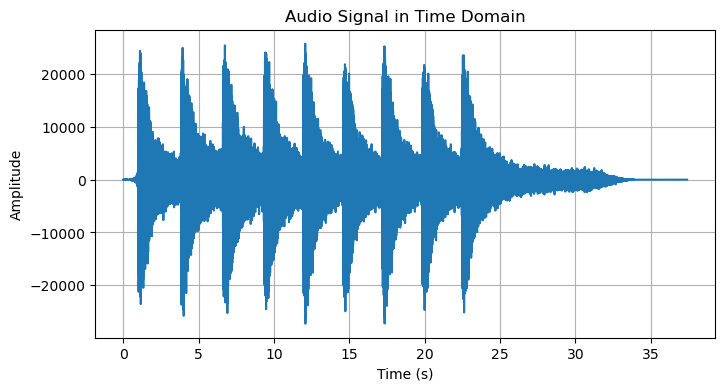
\includegraphics[keepaspectratio,alt={png}]{../images/notes-Using-FFTs_notes-Using-FFTs_tmp_5_0.png}}
\caption{png}
\end{figure}

\subsubsection{Fast Fourier Transform and the Power
Spectrum}\label{fast-fourier-transform-and-the-power-spectrum}

We can use the numpy FFT function to transform the time series into the
frequency domain. We can then plot the power spectrum. We have done this
before, but we made the signal ourselves. How do we choose how to break
down the signal? What is the \(dt\)?

The signal has a known sampling rate of 44.1 kHz; we get that from the
imported data information. This means that the time between samples is
\(dt = 1/44100\) s. We use the variable \texttt{sample\_rate} that we
defined above to calculate this.

Here, we also compute the power spectrum. We've made the choice to
sqaure the absoluate value of the FFT; this is a common choice to
represent power or intensity in some situtations. We also double the FFT
like before to deal with the negative frequencies. And we scale it by
the sum of the spectrum, which is another choice. We have done most of
this before and you can choose something else. The important thing is
the relative values of the power spectrum.

\begin{Shaded}
\begin{Highlighting}[]
\CommentTok{\# Calculate the two{-}sided power spectrum}
\NormalTok{data\_fft }\OperatorTok{=}\NormalTok{ fft(data)}
\NormalTok{power\_spectrum }\OperatorTok{=}\NormalTok{ np.}\BuiltInTok{abs}\NormalTok{(data\_fft)}\OperatorTok{**}\DecValTok{2}

\NormalTok{freqs }\OperatorTok{=}\NormalTok{ np.fft.fftfreq(}\BuiltInTok{len}\NormalTok{(data\_fft), }\DecValTok{1}\OperatorTok{/}\NormalTok{sample\_rate)}

\CommentTok{\# Convert to a one{-}sided power spectrum by taking the first half and doubling it}
\NormalTok{one\_sided\_power\_spectrum }\OperatorTok{=}\NormalTok{ power\_spectrum[:num\_samples}\OperatorTok{//}\DecValTok{2}\NormalTok{] }\OperatorTok{*} \DecValTok{2} \OperatorTok{/}\NormalTok{ np.}\BuiltInTok{sum}\NormalTok{(power\_spectrum)}
\NormalTok{one\_sided\_power\_spectrum[}\DecValTok{0}\NormalTok{] }\OperatorTok{/=} \DecValTok{2}  \CommentTok{\# Do not double the DC component}
\end{Highlighting}
\end{Shaded}

\begin{Shaded}
\begin{Highlighting}[]
\CommentTok{\# Plot the normalized one{-}sided power spectrum}
\NormalTok{plt.figure(figsize}\OperatorTok{=}\NormalTok{(}\DecValTok{8}\NormalTok{, }\DecValTok{4}\NormalTok{))}

\NormalTok{plt.plot(freqs[:num\_samples}\OperatorTok{//}\DecValTok{2}\NormalTok{], one\_sided\_power\_spectrum)}
\NormalTok{plt.xlim(}\DecValTok{0}\NormalTok{, }\DecValTok{5000}\NormalTok{)}

\NormalTok{plt.title(}\StringTok{\textquotesingle{}Power Spectrum of an Audio Signal\textquotesingle{}}\NormalTok{)}
\NormalTok{plt.xlabel(}\StringTok{\textquotesingle{}Frequency (Hz)\textquotesingle{}}\NormalTok{)}
\NormalTok{plt.ylabel(}\StringTok{\textquotesingle{}Power (Arb. Units)\textquotesingle{}}\NormalTok{)}

\NormalTok{plt.grid()}
\end{Highlighting}
\end{Shaded}

\begin{figure}
\centering
\pandocbounded{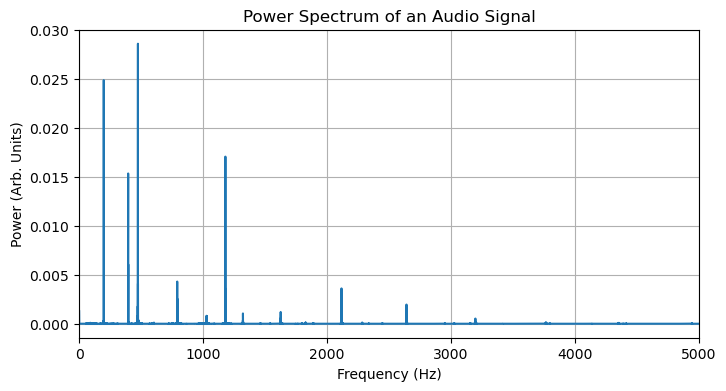
\includegraphics[keepaspectratio,alt={png}]{../images/notes-Using-FFTs_notes-Using-FFTs_tmp_8_0.png}}
\caption{png}
\end{figure}

\paragraph{Finding the peaks}\label{finding-the-peaks}

We see that we can find the frequencies of the peaks in the power
spectrum. It might seem hard to pick them out. That is because the scale
changes wildly. We can use a log scale to make it easier to see the
peaks. Below we do that and you see many more peaks.

\begin{Shaded}
\begin{Highlighting}[]
\NormalTok{plt.figure(figsize}\OperatorTok{=}\NormalTok{(}\DecValTok{8}\NormalTok{, }\DecValTok{4}\NormalTok{))}

\NormalTok{plt.plot(freqs[:num\_samples}\OperatorTok{//}\DecValTok{2}\NormalTok{], np.log(one\_sided\_power\_spectrum))}
\NormalTok{plt.xlim(}\DecValTok{0}\NormalTok{, }\DecValTok{5000}\NormalTok{)}

\NormalTok{plt.xlabel(}\StringTok{\textquotesingle{}Frequency (Hz)\textquotesingle{}}\NormalTok{)}
\NormalTok{plt.ylabel(}\StringTok{\textquotesingle{}Log(Power)\textquotesingle{}}\NormalTok{)}

\NormalTok{plt.grid()}
\end{Highlighting}
\end{Shaded}

\begin{figure}
\centering
\pandocbounded{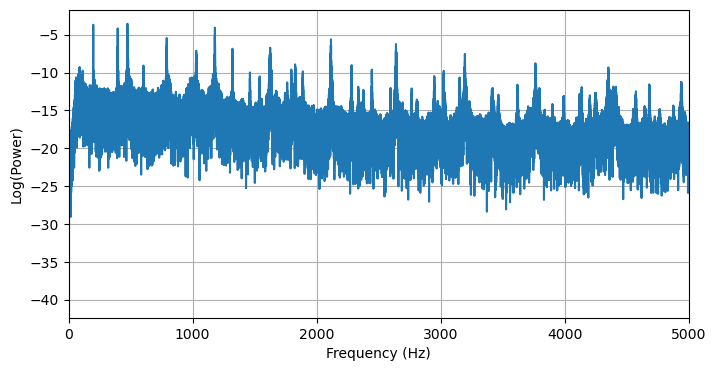
\includegraphics[keepaspectratio,alt={png}]{../images/notes-Using-FFTs_notes-Using-FFTs_tmp_10_0.png}}
\caption{png}
\end{figure}

\textbf{✅ Try this}

Look up the
\href{https://docs.scipy.org/doc/scipy/reference/generated/scipy.signal.find_peaks.html}{\texttt{find\_peaks}}
function from the \texttt{scipy.signal} library and try to find the
frequency peaks. Which notes are closest to the peaks?

\begin{Shaded}
\begin{Highlighting}[]
\CommentTok{\#\# Your code here}
\end{Highlighting}
\end{Shaded}

\subsection{Images}\label{images}

Many physics experiments use image data to record their results. This is
especially true in astronomy. We can use the FFT to analyze images.
Imaging enhancement can take the form of many different techniques, but
will illustrate a classic one called the Gaussian filter. For this
example, we will use an image from the
\href{https://en.wikipedia.org/wiki/Hubble_Deep_Field}{Hubble Ultra Deep
Field}. You can see a color version below:

\begin{figure}
\centering
\pandocbounded{\includegraphics[keepaspectratio,alt={Hubble Ultra Deep Field}]{https://images-assets.nasa.gov/image/GSFC_20171208_Archive_e001061/GSFC_20171208_Archive_e001061~small.jpg}}
\caption{Hubble Ultra Deep Field}
\end{figure}

We can load the image as grey scale. Here the matrix represents the
intensity of the light at each pixel. We can plot the image. We see that
it is a bit noisy. We can use the FFT to filter out some of the noise.

\begin{Shaded}
\begin{Highlighting}[]
\NormalTok{image }\OperatorTok{=}\NormalTok{ Image.}\BuiltInTok{open}\NormalTok{(}\StringTok{\textquotesingle{}../assets/data/hubble.jpeg\textquotesingle{}}\NormalTok{).convert(}\StringTok{\textquotesingle{}L\textquotesingle{}}\NormalTok{)  }\CommentTok{\# Convert to grayscale}
\NormalTok{plt.imshow(image, cmap}\OperatorTok{=}\StringTok{\textquotesingle{}gray\textquotesingle{}}\NormalTok{)}
\end{Highlighting}
\end{Shaded}

\begin{verbatim}
<matplotlib.image.AxesImage at 0x139355e20>
\end{verbatim}

\begin{figure}
\centering
\pandocbounded{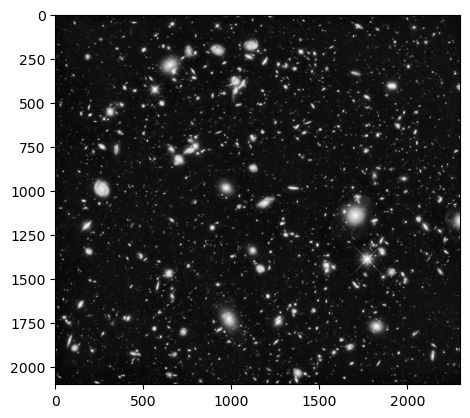
\includegraphics[keepaspectratio,alt={png}]{../images/notes-Using-FFTs_notes-Using-FFTs_tmp_14_1.png}}
\caption{png}
\end{figure}

\subsubsection{Reducing Noise}\label{reducing-noise}

There are many applications of the FFT to image processing, but one is
\href{https://en.wikipedia.org/wiki/Noise_reduction}{noise reduction}.
We can use the FFT to filter out some of the noise.

We will use a Gaussian filter. This is a common filter that is used in
many applications. It is a
\href{https://en.wikipedia.org/wiki/Convolution}{convolution} of the
image with a Gaussian function. We will use the
\href{https://docs.scipy.org/doc/scipy/reference/generated/scipy.ndimage.gaussian_filter.html}{\texttt{gaussian\_filter}}
function from the \texttt{scipy.ndimage} library. We don't expect you to
learn what this is in detail unless you start to investigate it for a
project. We will just use it here.

In class, we will do this kind of work in 1 dimension to clean and
filter signals. Below, we import the filter, and then proceed with the
FFT for the image; we filter it; and then we transform it back to the
image. We plot the original and the filtered image. You can see that the
noise is reduced yielding a clearer image.

\begin{Shaded}
\begin{Highlighting}[]
\ImportTok{from}\NormalTok{ scipy.ndimage }\ImportTok{import}\NormalTok{ gaussian\_filter}

\CommentTok{\#\# Convert the image to a numpy array}
\NormalTok{image\_array }\OperatorTok{=}\NormalTok{ np.array(image)}

\CommentTok{\# Apply 2D FFT and shift zero frequency components to the center of the spectrum}
\NormalTok{f\_transform }\OperatorTok{=}\NormalTok{ fftshift(fft2(image\_array))}

\CommentTok{\# Apply a Gaussian filter in the frequency domain for noise reduction (don\textquotesingle{}t worry too much about this, we\textquotesingle{}re just altering the magnitude spectrum)}
\NormalTok{f\_transform\_filtered }\OperatorTok{=}\NormalTok{ gaussian\_filter(np.}\BuiltInTok{abs}\NormalTok{(f\_transform), sigma}\OperatorTok{=}\DecValTok{5}\NormalTok{) }\OperatorTok{*}\NormalTok{ np.exp(}\OtherTok{1j} \OperatorTok{*}\NormalTok{ np.angle(f\_transform))}

\CommentTok{\# Calculate the magnitude spectra for plotting}
\NormalTok{magnitude\_spectrum }\OperatorTok{=}\NormalTok{ np.log(np.}\BuiltInTok{abs}\NormalTok{(f\_transform))}
\NormalTok{filtered\_magnitude\_spectrum }\OperatorTok{=}\NormalTok{ np.log(np.}\BuiltInTok{abs}\NormalTok{(f\_transform\_filtered))}

\CommentTok{\# Apply 2D inverse transform to get the noise{-}reduced image}
\NormalTok{image\_denoised }\OperatorTok{=}\NormalTok{ ifft2(fftshift(f\_transform\_filtered)).real}
\end{Highlighting}
\end{Shaded}

\begin{Shaded}
\begin{Highlighting}[]
\NormalTok{plt.figure(figsize}\OperatorTok{=}\NormalTok{(}\DecValTok{12}\NormalTok{, }\DecValTok{12}\NormalTok{))}

\NormalTok{plt.subplot(}\DecValTok{221}\NormalTok{), plt.imshow(image\_array, cmap}\OperatorTok{=}\StringTok{\textquotesingle{}gray\textquotesingle{}}\NormalTok{), plt.title(}\StringTok{\textquotesingle{}Original Image\textquotesingle{}}\NormalTok{)}
\NormalTok{plt.subplot(}\DecValTok{222}\NormalTok{), plt.imshow(magnitude\_spectrum, cmap}\OperatorTok{=}\StringTok{\textquotesingle{}gray\textquotesingle{}}\NormalTok{), plt.title(}\StringTok{\textquotesingle{}Magnitude Spectrum\textquotesingle{}}\NormalTok{)}
\NormalTok{plt.subplot(}\DecValTok{223}\NormalTok{), plt.imshow(image\_denoised, cmap}\OperatorTok{=}\StringTok{\textquotesingle{}gray\textquotesingle{}}\NormalTok{), plt.title(}\StringTok{\textquotesingle{}Denoised Image\textquotesingle{}}\NormalTok{)}
\NormalTok{plt.subplot(}\DecValTok{224}\NormalTok{), plt.imshow(filtered\_magnitude\_spectrum, cmap}\OperatorTok{=}\StringTok{\textquotesingle{}gray\textquotesingle{}}\NormalTok{), plt.title(}\StringTok{\textquotesingle{}Filtered Magnitude Spectrum\textquotesingle{}}\NormalTok{)}

\NormalTok{plt.tight\_layout()}
\end{Highlighting}
\end{Shaded}

\begin{figure}
\centering
\pandocbounded{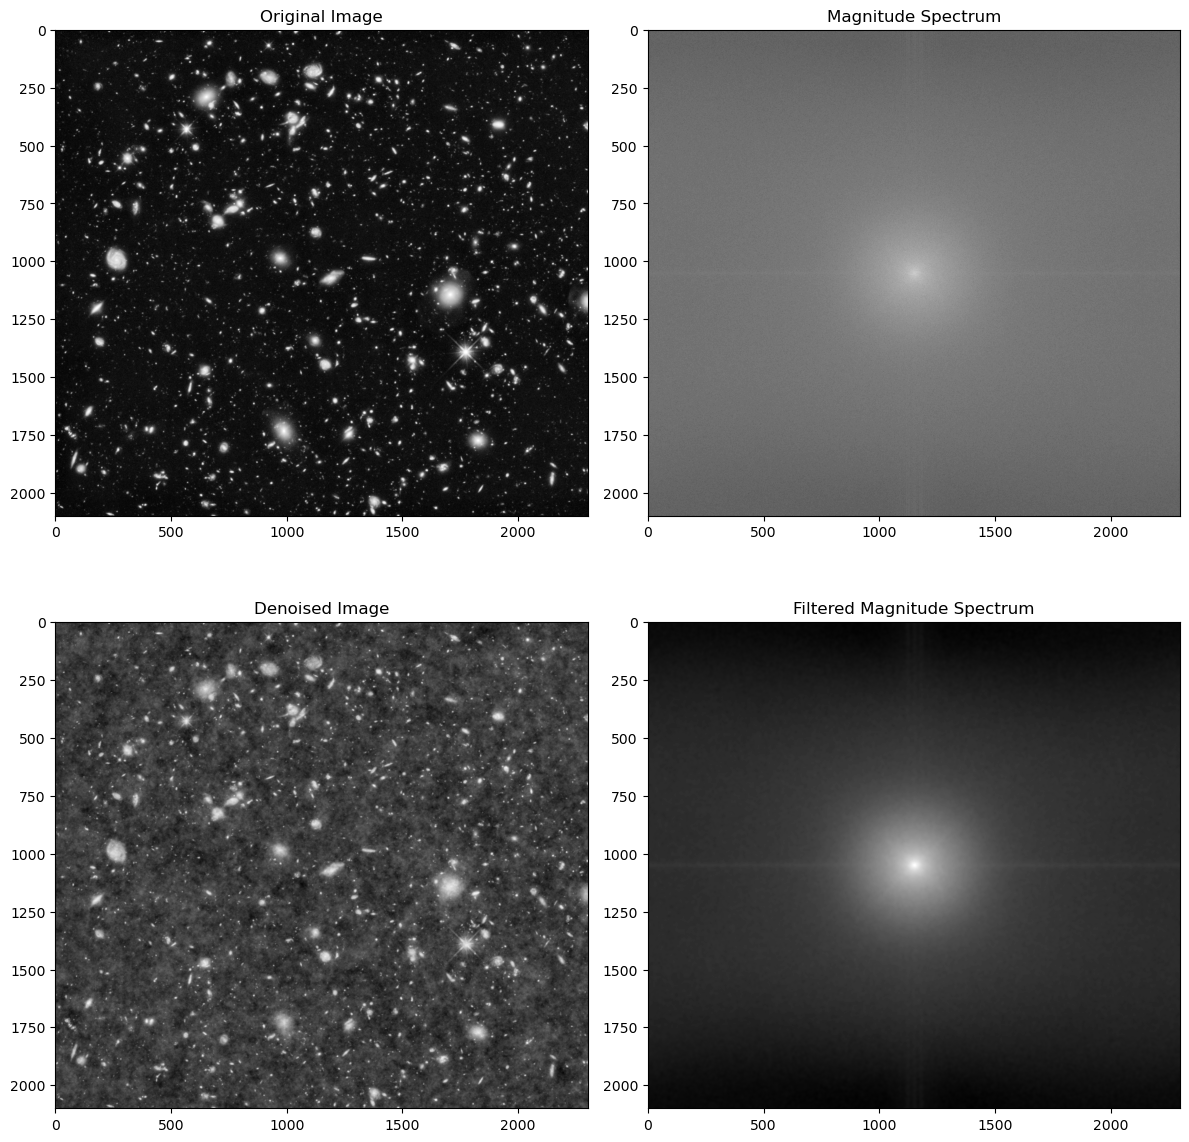
\includegraphics[keepaspectratio,alt={png}]{../images/notes-Using-FFTs_notes-Using-FFTs_tmp_17_0.png}}
\caption{png}
\end{figure}

The FFT is widely useful tool. We highlight only two applications here,
but there are many more. We will use the FFT in class to analyze signals
and images.
